% !TeX root = ../MQF_Manuale_Master.tex
% Capitoli/MQF_Cap_15_Programmazione_Stocastica_II_v2.tex

\chapter{Soluzione e valore dell'informazione}

\label{cap:soluzione-valore-informazione-v2}

\medskip

Il Capitolo~\ref{cap:programmazione-stocastica-due-stadi} ha introdotto il
programma stocastico lineare a due stadi. La decisione iniziale $x$ viene
assunta prima di conoscere quale scenario si realizzer\`a. Dopo
l'osservazione dello scenario $s$, il decisore pu\`o invece adattare il piano
attraverso una decisione di ricorso $y_s$.

Con un insieme finito di scenari, il problema \`e stato scritto nella forma

\[
\max_{x\in\mathcal X}
\left\{
c'x+
\sum_{s\in\mathcal S}p_sQ_s(x)
\right\},
\]

dove $Q_s(x)$ \`e il valore ottimo del problema di secondo stadio nello
scenario $s$.
Questa formulazione chiarisce la struttura fondamentale di una decisione
sotto incertezza, ma lascia aperte alcune questioni che riguardano direttamente
la soluzione del problema.

La prima \`e una questione di fattibilit\`a. Una decisione $x$ ammissibile al
primo stadio non garantisce, in generale, che esista una decisione di ricorso
ammissibile in ogni scenario. Prima di attribuire un significato economico a
$Q_s(x)$ occorre quindi verificare che il problema di secondo stadio possa
effettivamente essere risolto. Questo problema sar\`a affrontato nella
Sezione~\ref{sec:cap15-fattibilita-ricorso-v2}.

La seconda questione riguarda la dipendenza del ricorso dalla decisione
iniziale. Scegliere $x$ significa infatti determinare le risorse e i vincoli
con i quali il decisore affronter\`a gli scenari futuri. Decisioni iniziali
diverse generano quindi, in generale, problemi di secondo stadio diversi e
valori diversi di $Q_s(x)$. Nel caso lineare questa dipendenza presenta una
struttura precisa, studiata nella
Sezione~\ref{sec:cap15-proprieta-funzione-ricorso-v2}.

Indicheremo con

\[
x^{SP}
\]

la soluzione ottima del programma stocastico e con

\[
z^{SP}
\]

il corrispondente valore ottimo.

La soluzione $x^{SP}$ non \`e la decisione migliore per uno specifico
scenario. \`E una decisione unica, assunta prima che l'incertezza venga
rivelata, che tiene conto congiuntamente degli scenari considerati, delle loro
probabilit\`a e delle possibilit\`a di adattamento disponibili dopo la loro
osservazione.

Questo punto \`e essenziale. La programmazione stocastica non sceglie oggi
ci\`o che sarebbe ottimo conoscendo gi\`a il futuro. Cerca invece la migliore
decisione compatibile con l'informazione disponibile nel momento in cui essa
deve essere assunta.

\medskip

\noindent
\textbf{Domanda guida:} quali propriet\`a deve possedere una decisione
stocastica, come si determina il compromesso tra scenari differenti e quanto
vale disporre di una migliore informazione sul futuro?

\medskip

Le prime sezioni del capitolo rispondono a queste domande restando ancora nel
quadro a due stadi. Dopo avere studiato la fattibilit\`a e le propriet\`a
della funzione di ricorso, confronteremo la soluzione stocastica con soluzioni
costruite sotto ipotesi informative differenti. Questo consentir\`a di
distinguere il valore prodotto dall'uso esplicito della distribuzione degli
scenari dal valore attribuibile a una conoscenza pi\`u completa del futuro.

Il modello a due stadi incorpora per\`o una struttura informativa molto
specifica: la decisione iniziale viene presa senza conoscere lo scenario
futuro, mentre l'intero blocco di ricorso viene formulato dopo che
l'incertezza rilevante \`e stata osservata.

Molti problemi finanziari hanno una struttura informativa pi\`u articolata.
L'informazione arriva progressivamente e l'orizzonte successivo alla
decisione iniziale pu\`o essere suddiviso in pi\`u stadi decisionali.

La decisione iniziale continua a essere indicata con $x$ ed \`e assunta al
tempo $t=0$, prima della rivelazione dell'incertezza futura. Come nel modello
a due stadi, essa \`e quindi comune a tutti gli scenari.

La differenza riguarda le decisioni successive. Nel modello a due stadi tutte
le decisioni di ricorso sono raccolte in un unico vettore $y_s$. Nel modello
multistadio, invece, l'orizzonte \`e suddiviso in $K$ stadi e le decisioni di
ricorso sono distinte come

\[
y_1^s,\ldots,y_K^s.
\]

Uno stadio pu\`o comprendere uno o pi\`u tempi del modello. L'insieme ordinato
dei tempi appartenenti allo stadio $k$ \`e indicato con

\[
\mathcal T_k
=
\{t_{k,1},\ldots,t_{k,n_k}\},
\]

mentre il suo tempo terminale \`e

\[
\bar t_k
=
t_{k,n_k}.
\]

La struttura multistadio conserva il principio informativo gi\`a presente
nel modello a due stadi. La differenza riguarda il numero di stadi nei quali
il ricorso viene distribuito lungo l'orizzonte.

\begin{center}
\begin{tabular}{|p{2.8cm}|p{3.7cm}|p{3.7cm}|}
\hline
 & \textbf{Modello a due stadi} & \textbf{Modello multistadio} \\
\hline
\raggedright Decisione iniziale
&
$x$, comune a tutti gli scenari
&
$x$, comune a tutti gli scenari
\\
\hline
\raggedright Decisione di ricorso
&
$y_s$
&
$y_k^s$, \quad $k=1,\ldots,K$
\\
\hline
\raggedright Condizione di adattamento
&
$y_s$ adattata a $\mathcal F_T$
&
$y_k^s$ adattata a $\mathcal F_{\bar t_k}$
\\
\hline
\end{tabular}
\end{center}

Ci\`o che cambia non \`e dunque la logica del ricorso, ma la struttura
temporale con cui essa viene applicata. Nel modello a due stadi esiste un
unico momento di adattamento successivo alla decisione iniziale; nel modello
multistadio il ricorso viene invece distribuito lungo l'orizzonte attraverso
pi\`u stadi decisionali.

Il vantaggio della formulazione multistadio consiste proprio in questa
maggiore capacit\`a di adattamento. Le decisioni possono essere aggiornate
progressivamente al procedere dell'informazione, anzich\`e concentrare
l'intero aggiustamento in un unico secondo stadio. Questo vantaggio richiede,
come contropartita, una rappresentazione pi\`u accurata della sequenza con cui
informazione e decisioni si succedono. Il passaggio dal modello a due stadi
al modello multistadio sar\`a sviluppato nella
Sezione~\ref{sec:cap15-motivazione-multistadio-v2}.

La formulazione generale del programma multistadio sar\`a poi introdotta
nella Sezione~\ref{sec:cap15-programma-multistadio-v2}.

Il caso guida SVB--ALM accompagner\`a questa costruzione con funzione
illustrativa. Nel modello a due stadi, $x^{SP}$ rappresenta una composizione
iniziale dell'attivo comune a tutte le possibili evoluzioni future, mentre
le decisioni di liquidit\`a e funding costituiscono il ricorso successivo.
Nel modello multistadio, tali decisioni possono invece essere aggiornate
progressivamente nei diversi stadi, in funzione dell'informazione disponibile.

Il caso guida servir\`a quindi a mostrare come le strutture matematiche
introdotte si traducano in un problema finanziario concreto, senza modificare
la natura generale del metodo. Fattibilit\`a del ricorso, struttura
informativa delle decisioni e adattamento progressivo restano propriet\`a
della programmazione stocastica, non del particolare problema ALM utilizzato
per illustrarle.

La parte conclusiva del capitolo torner\`a infine alla struttura
computazionale del problema e al principio della decomposizione, mostrando
come la struttura del ricorso possa essere sfruttata anche sul piano
risolutivo.

\medskip

\noindent
\textbf{Obiettivi della lezione.}

Al termine del capitolo lo studente dovr\`a essere in grado di:

\begin{itemize}

\item analizzare la fattibilit\`a del ricorso, le principali propriet\`a
della funzione di ricorso e il ruolo congiunto della decisione iniziale e
delle decisioni di ricorso nei diversi scenari;

\item costruire e confrontare soluzione stocastica, Expected Value e
wait-and-see, interpretando il significato economico di $\EVPI$ e $\VSS$;

\item comprendere il passaggio dal modello a due stadi al modello multistadio,
formalizzando l'adattamento progressivo delle decisioni all'informazione
disponibile e il principio di non anticipativit\`a;

\item distinguere le principali rappresentazioni del problema multistadio e
riconoscere la struttura che consente di formulare il problema mediante alberi
degli scenari, stati sufficienti e metodi di decomposizione.

\end{itemize}

\section{Fattibilit\`a del ricorso}

\label{sec:cap15-fattibilita-ricorso-v2}

Nel programma stocastico a due stadi introdotto nel
Capitolo~\ref{cap:programmazione-stocastica-due-stadi}, la decisione iniziale
$x$ viene scelta tenendo conto delle migliori decisioni di ricorso disponibili
nei diversi scenari.

Prima di studiare il valore economico del ricorso occorre tuttavia risolvere
una questione preliminare: una volta fissata $x$ e osservato lo scenario $s$,
esiste almeno una decisione di secondo stadio che soddisfa i vincoli del
problema?

Per lo scenario $s$, il problema di ricorso \`e

\[
Q_s(x)
=
\max_{y_s\in\mathcal X_s}
\left\{
q_s'y_s:
T_sx+W_sy_s=h_s
\right\}.
\]

La quantit\`a $Q_s(x)$ rappresenta il valore della migliore risposta
disponibile nello scenario $s$, ma tale valore pu\`o essere definito come
valore ottimo del problema di secondo stadio soltanto quando l'insieme delle
decisioni di ricorso ammissibili $\mathcal X_s$ non \`e vuoto.

\begin{definition}[Ricorso ammissibile]

Fissati una decisione di primo stadio $x\in\mathcal X$ e uno scenario
$s\in\mathcal S$, il ricorso \`e \emph{ammissibile} se esiste almeno una
decisione

\[
y_s\in\mathcal X_s
\]

tale che

\[
T_sx+W_sy_s=h_s.
\]

\end{definition}

La definizione riguarda una specifica coppia $(x,s)$. Una decisione iniziale
pu\`o quindi ammettere ricorso in uno scenario e non ammetterlo in un altro.
Inoltre, la fattibilit\`a non dice ancora nulla sulla convenienza economica
della risposta: due decisioni iniziali possono entrambe ammettere ricorso e
produrre valori di $Q_s(x)$ molto diversi.

Occorre ora distinguere questa propriet\`a locale da due propriet\`a pi\`u
generali della struttura di ricorso.

\begin{definition}[Ricorso completo]

Il problema possiede \emph{ricorso completo} se, per ogni possibile vettore
$b$ compatibile con le dimensioni del sistema di secondo stadio, esiste una
decisione di ricorso ammissibile tale che

\[
W_sy_s=b.
\]

Equivalentemente, nella relazione

\[
W_sy_s=h_s-T_sx,
\]

la struttura di ricorso \`e in grado di soddisfare qualunque possibile valore
del termine noto.

\end{definition}

Il ricorso completo \`e quindi una propriet\`a della capacit\`a correttiva
offerta dal secondo stadio. Non si limita ai valori di $h_s-T_sx$ che possono
effettivamente verificarsi nel modello, ma richiede che il sistema di ricorso
sia in grado di compensare un termine noto arbitrario.

Questa condizione \`e spesso pi\`u forte di quanto sia necessario nelle
applicazioni. Per la soluzione del programma stocastico interessa infatti
soprattutto sapere se il ricorso \`e possibile per le decisioni di primo
stadio e per gli scenari che il modello considera effettivamente.

\begin{definition}[Ricorso relativamente completo]

Un programma stocastico a due stadi possiede
\emph{ricorso relativamente completo} se, per ogni decisione ammissibile di
primo stadio

\[
x\in\mathcal X
\]

e per ogni scenario

\[
s\in\mathcal S,
\]

esiste almeno una decisione di ricorso

\[
y_s\in\mathcal X_s
\]

tale che

\[
T_sx+W_sy_s=h_s.
\]

\end{definition}

La differenza tra le due propriet\`a riguarda dunque l'insieme dei termini
noti per i quali viene richiesta la fattibilit\`a del secondo stadio. Il
ricorso completo considera tutti i termini noti possibili; il ricorso
relativamente completo considera soltanto quelli generati dalle decisioni
ammissibili $x\in\mathcal X$ e dagli scenari inclusi nel modello.

\begin{center}
\begin{tabular}{p{3.5cm}p{8.0cm}}
\hline
\textbf{Propriet\`a} & \textbf{Condizione richiesta} \\
\hline

\emph{Ricorso completo}
&
Il secondo stadio \`e ammissibile per qualunque possibile termine noto del
sistema di ricorso.
\\[4pt]

\emph{Ricorso relativamente completo}
&
Il secondo stadio \`e ammissibile per tutti i termini noti effettivamente
generati da $x\in\mathcal X$ e dagli scenari del modello.
\\
\hline
\end{tabular}
\end{center}

Il ricorso completo implica quindi il ricorso relativamente completo, ma non
vale in generale il contrario. Quest'ultima propriet\`a dipende infatti anche
dall'insieme $\mathcal X$ e dagli scenari considerati: restringendo l'insieme
delle decisioni ammissibili di primo stadio si pu\`o ottenere ricorso
relativamente completo anche quando la struttura di secondo stadio non
possiede ricorso completo.

Nel caso ALM la distinzione ha un'interpretazione immediata. La banca dispone
di strumenti di riequilibrio, come la raccolta di nuovo funding, ma tali
strumenti possono essere soggetti a limiti di capacit\`a. Non \`e quindi
necessario n\'e realistico richiedere che qualsiasi deficit di liquidit\`a
immaginabile possa essere compensato. Occorre invece verificare che tutte le
decisioni iniziali considerate ammissibili lascino una capacit\`a di
correzione sufficiente negli scenari inclusi nel modello.

\subsection{Un esempio con capacit\`a limitata di funding}

Consideriamo un problema ridotto con due classi di attivo e risorse iniziali

\[
A_0=10.
\]

Indichiamo con $x$ l'ammontare investito nella classe di attivo pi\`u liquida.
La composizione iniziale \`e pertanto

\[
\begin{pmatrix}
x\\
10-x
\end{pmatrix},
\qquad
0\leq x\leq10.
\]

Alla data di ricorso deve essere soddisfatto un fabbisogno di liquidit\`a

\[
d=8.
\]

Consideriamo due scenari. Nello scenario ordinario, i coefficienti che
trasformano le due posizioni iniziali in liquidit\`a disponibile sono

\[
a_1'
=
(1,\;0.6),
\]

mentre nello scenario avverso sono

\[
a_2'
=
(1,\;0.2).
\]

La prima classe mantiene quindi la propria capacit\`a di generare liquidit\`a,
mentre la seconda diventa molto meno efficace nello scenario avverso.

Dopo l'osservazione dello scenario la banca pu\`o utilizzare nuovo funding
$u_s$ e mantenere un'eventuale giacenza residua $g_s$, con

\[
g_s\geq0,
\qquad
0\leq u_s\leq\bar u_s.
\]

Le capacit\`a massime di funding sono

\[
\bar u_1=1,
\qquad
\bar u_2=2.
\]

Il bilancio di secondo stadio \`e

\[
a_s'
\begin{pmatrix}
x\\
10-x
\end{pmatrix}
+
u_s
=
8+g_s.
\]

Poich\`e $g_s\geq0$, il funding minimo necessario nello scenario $s$ coincide
con il deficit di liquidit\`a quando tale deficit \`e positivo.

Nello scenario ordinario la liquidit\`a generata dagli attivi \`e

\[
x+0.6(10-x)
=
6+0.4x.
\]

Il funding minimo richiesto \`e quindi

\[
u_1^{\min}(x)
=
\max\{0,\;2-0.4x\}.
\]

Il ricorso \`e ammissibile se

\[
u_1^{\min}(x)
\leq
\bar u_1=1,
\]

ossia se

\[
x\geq2.5.
\]

Nello scenario avverso la liquidit\`a disponibile \`e invece

\[
x+0.2(10-x)
=
2+0.8x,
\]

da cui

\[
u_2^{\min}(x)
=
\max\{0,\;6-0.8x\}.
\]

La condizione

\[
u_2^{\min}(x)
\leq
\bar u_2=2
\]

richiede

\[
x\geq5.
\]

Lo scenario avverso impone quindi il requisito pi\`u severo sulla decisione
iniziale.

Per esempio, se

\[
x=4,
\]

nello scenario ordinario si ha

\[
u_1^{\min}(4)=0.4<1,
\]

e il ricorso \`e ammissibile. Nello scenario avverso, invece,

\[
u_2^{\min}(4)=2.8>2.
\]

La capacit\`a massima di funding non \`e sufficiente e il problema di secondo
stadio non ammette soluzioni. La stessa decisione iniziale risulta quindi
compatibile con uno scenario ma non con l'altro.

Se invece

\[
x=6,
\]

si ottiene

\[
u_1^{\min}(6)=0
\]

nello scenario ordinario e

\[
u_2^{\min}(6)=1.2<2
\]

nello scenario avverso. La decisione $x=6$ ammette quindi ricorso in entrambi
gli scenari.

La Figura~\ref{fig:cap15-fattibilita-ricorso-v2} mostra il risultato per tutti
i valori di $x$ compresi tra $0$ e $10$.

\begin{figure}[htbp]
\centering
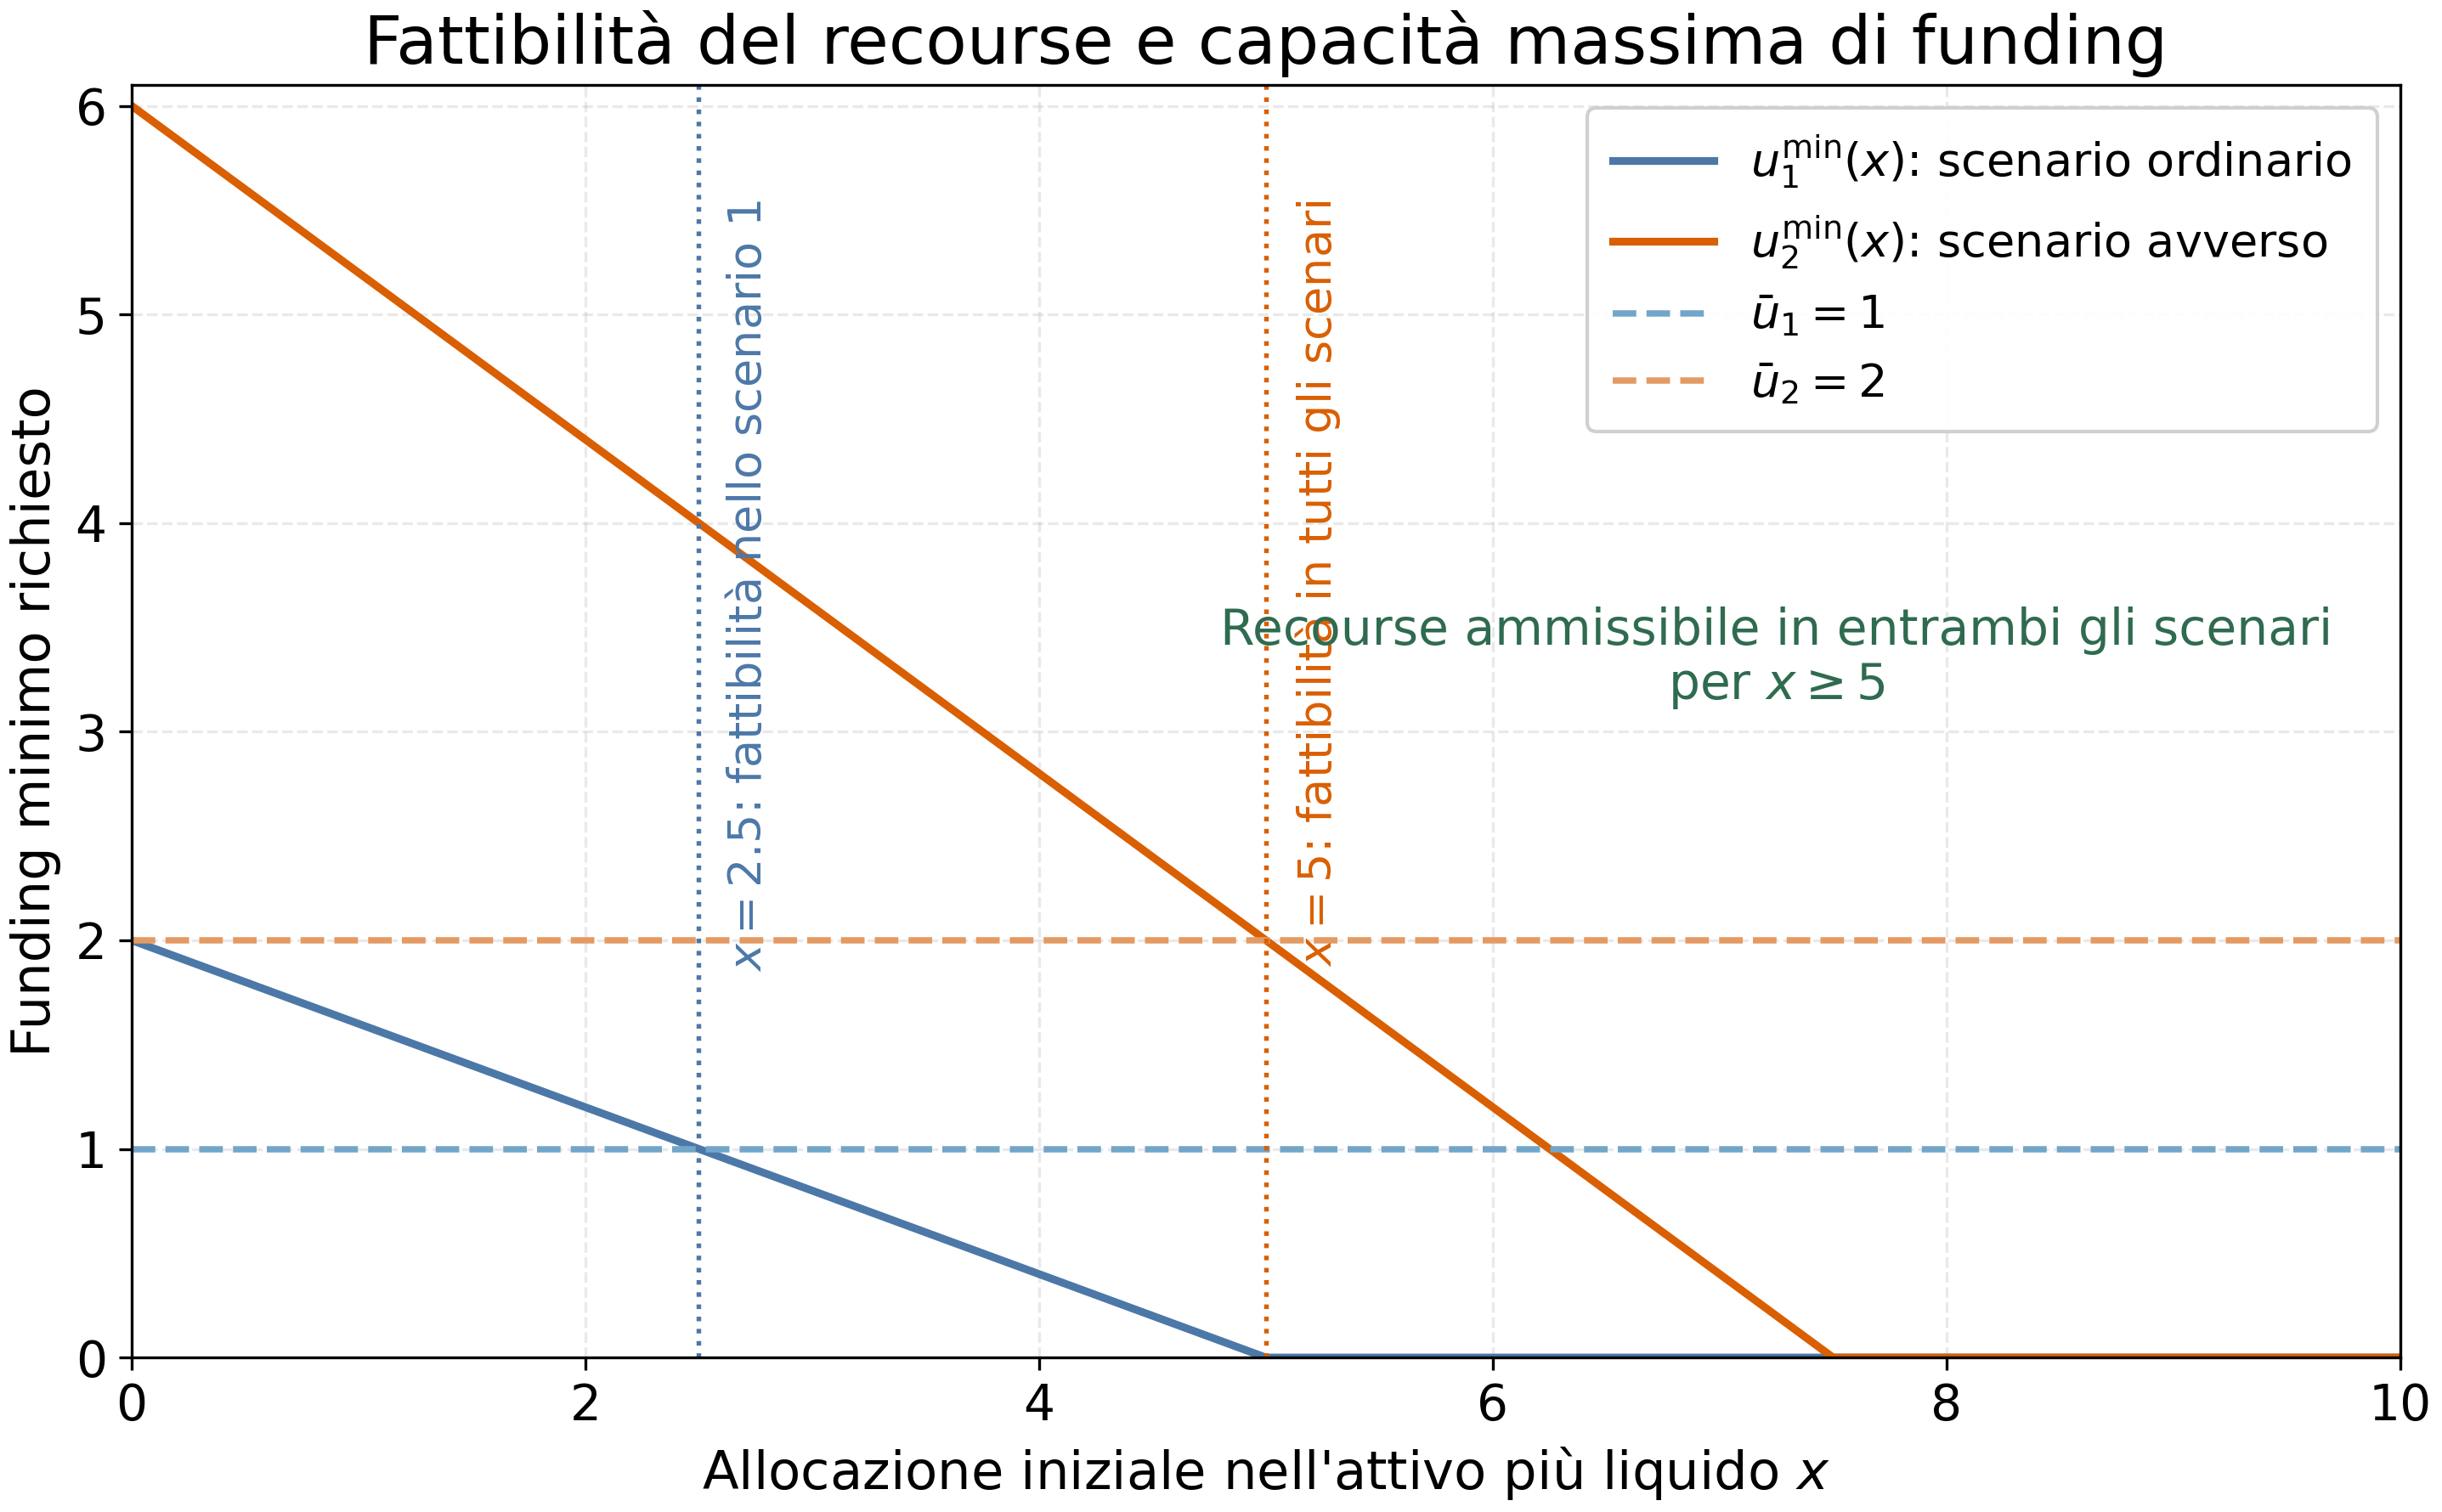
\includegraphics[width=0.94\textwidth]
{../graphics/Cap15_fattibilita_ricorso.png}
\caption{Funding minimo richiesto nei due scenari al variare
dell'allocazione iniziale nella classe di attivo pi\`u liquida.
L'intersezione tra $u_s^{\min}(x)$ e la corrispondente capacit\`a massima
$\bar u_s$ individua la soglia oltre la quale il ricorso diventa ammissibile
nello scenario. Per $x\geq5$ il problema di secondo stadio \`e ammissibile in
entrambi gli scenari.}
\label{fig:cap15-fattibilita-ricorso-v2}
\end{figure}

La figura individua tre regioni. Per

\[
0\leq x<2.5,
\]

la capacit\`a di funding non \`e sufficiente nemmeno nello scenario ordinario.
Per

\[
2.5\leq x<5,
\]

il ricorso \`e ammissibile nello scenario ordinario ma non in quello avverso.
Infine, per

\[
x\geq5,
\]

entrambi i problemi di secondo stadio sono ammissibili.

L'esempio consente anche di distinguere le due propriet\`a generali appena
definite. Se

\[
\mathcal X=[0,10],
\]

il modello non possiede ricorso relativamente completo, perch\`e esistono
decisioni ammissibili di primo stadio, come $x=4$, che rendono inammissibile
il ricorso in almeno uno scenario.

Se invece ulteriori vincoli di primo stadio restringono l'insieme a

\[
\mathcal X=[5,10],
\]

allora ogni $x\in\mathcal X$ ammette ricorso in entrambi gli scenari e il
problema possiede ricorso relativamente completo.

Ci\`o non implica ricorso completo. La capacit\`a di funding resta limitata:
un deficit sufficientemente elevato non potrebbe essere compensato da alcuna
decisione $u_s\leq\bar u_s$. La struttura di ricorso non \`e quindi in grado
di soddisfare un termine noto arbitrario.

Nel caso SVB--ALM completo lo stesso meccanismo opera attraverso pi\`u date,
pi\`u classi di attivo e pi\`u limiti di funding. Una composizione iniziale
pu\`o essere ammissibile al primo stadio ma lasciare la banca incapace di
soddisfare uno dei successivi bilanci di liquidit\`a in uno scenario severo.

La fattibilit\`a costituisce quindi il primo filtro nella valutazione di una
decisione stocastica. Soltanto dopo avere verificato l'esistenza delle
decisioni di ricorso ha senso studiarne il valore economico. La sezione
successiva analizza come la funzione $Q_s(x)$ varia al variare della decisione
iniziale.

\section{Propriet\`a della funzione di ricorso}

\label{sec:cap15-proprieta-funzione-ricorso-v2}

La sezione precedente ha mostrato che il valore del ricorso pu\`o essere
studiato soltanto quando il problema di secondo stadio \`e ammissibile.
Assumiamo ora che questa condizione sia soddisfatta e consideriamo la funzione
di ricorso introdotta nella
\eqref{eq:cap14-ricorso-scenario}:

\[
Q_s(x)
=
\max_{y_s\in\mathcal X_s}
\left\{
q_s'y_s:
T_sx+W_sy_s=h_s
\right\}.
\]

Per ogni decisione iniziale $x$, la quantit\`a $Q_s(x)$ rappresenta il valore
ottimo della migliore risposta disponibile dopo l'osservazione dello
scenario $s$. La funzione di ricorso descrive quindi come il valore delle
possibilit\`a di adattamento future dipenda dalla decisione presa al primo
stadio.

\subsection{Dipendenza dalla decisione iniziale}

Una volta fissato lo scenario $s$, la decisione iniziale $x$ entra nei vincoli
del problema di ricorso attraverso il termine

\[
h_s-T_sx.
\]

Modificare $x$ significa pertanto modificare le condizioni nelle quali il
secondo stadio dovr\`a operare. In un problema di gestione della liquidit\`a,
per esempio, una composizione iniziale pi\`u liquida pu\`o ridurre il deficit
da finanziare negli scenari avversi; una composizione meno liquida pu\`o
invece aumentare il ricorso al funding.

Per due decisioni iniziali

\[
x'
\qquad\text{e}\qquad
x'',
\]

si ottengono quindi, in generale, valori differenti

\[
Q_s(x')
\qquad\text{e}\qquad
Q_s(x'').
\]

La qualit\`a della decisione iniziale non pu\`o essere valutata considerando
soltanto il contributo diretto $c'x$: occorre tenere conto anche dell'effetto
che $x$ produce sul valore delle decisioni di ricorso disponibili nei diversi
scenari.

\subsection{Struttura nel caso lineare}

Nel programma stocastico lineare a due stadi, questa dipendenza possiede una
struttura particolarmente regolare.

\begin{proposition}

Si consideri, per uno scenario fissato $s$, la funzione

\[
Q_s(x)
=
\max_{y_s\in\mathcal X_s}
\left\{
q_s'y_s:
T_sx+W_sy_s=h_s
\right\}.
\]

Se il problema di secondo stadio \`e ammissibile per i valori di $x$
considerati e possiede valore ottimo finito, allora $Q_s(x)$ \`e concava e
lineare a tratti rispetto a $x$ sul proprio dominio di fattibilit\`a.

\end{proposition}

Il risultato deriva dalla struttura parametrica del problema lineare.
Fissato lo scenario, $x$ modifica il termine noto

\[
h_s-T_sx,
\]

mentre la struttura del problema di secondo stadio rimane lineare. Il valore
ottimo varia quindi per tratti lineari al variare di $x$. Poich\`e il
problema di ricorso \`e formulato come una massimizzazione, la funzione
risultante \`e concava rispetto alla decisione iniziale $x$ sul
proprio dominio di fattibilit\`a..

I punti nei quali cambia la pendenza di $Q_s(x)$ corrispondono a cambiamenti
nella struttura della soluzione ottima del problema di secondo stadio. 
La linearit\`a a tratti implica che il valore marginale di una variazione di $x$ sia costante all'interno di ciascun tratto lineare, ma in generale cambi
quando si passa da un tratto all'altro.

Questa propriet\`a ha anche un'importante conseguenza computazionale: la
struttura lineare a tratti della funzione di ricorso \`e uno degli elementi
che rendono possibile sfruttare separatamente i problemi di secondo stadio
nei metodi di decomposizione. Questo aspetto verr\`a ripreso nella parte
conclusiva del capitolo.

\subsection{Un esempio unidimensionale}

Consideriamo un problema ALM ridotto a due classi di attivo. Il patrimonio
inizialmente allocabile \`e

\[
A_0=10\,000
\]

milioni di euro. Indichiamo con $x_1$ l'investimento nell'attivo pi\`u
liquido e con $x_2$ l'investimento nell'attivo meno liquido. L'intero
patrimonio viene investito:

\[
x_1+x_2=10\,000,
\qquad
x_1,x_2\geq0.
\]

Consideriamo lo scenario avverso $s=2$. Alla data di ricorso, l'attivo
pi\`u liquido rende disponibile integralmente il capitale investito, mentre
dell'attivo meno liquido \`e disponibile soltanto il $20\%$ del valore
iniziale. La liquidit\`a generata dal portafoglio \`e quindi

\[
L_2
=
x_1+0.2x_2.
\]

Il coefficiente $0.2$ rappresenta la quota dell'investimento disponibile
alla data in cui deve essere soddisfatto il fabbisogno di liquidit\`a; non
rappresenta il rendimento dell'attivo.

Supponiamo che il fabbisogno sia

\[
d=6\,000
\]

milioni di euro. La banca pu\`o raccogliere nuovo funding $u_2\geq0$ oppure
mantenere come giacenza l'eventuale liquidit\`a eccedente, $g_2\geq0$. Il
bilancio di secondo stadio \`e

\[
x_1+0.2x_2+u_2
=
6\,000+g_2.
\]

Assumiamo che il funding abbia un costo complessivo pari al $3\%$
dell'ammontare raccolto. Il problema di ricorso nello scenario avverso
diventa

\[
Q_2(x)
=
\max_{g_2,u_2\geq0}
\left\{
-0.03u_2:
x_1+0.2x_2+u_2=6\,000+g_2
\right\}.
\]

Poich\`e il problema complessivo \`e formulato come una massimizzazione, il
costo del funding entra nella funzione di ricorso con segno negativo. Se

\[
C_2=0.03u_2,
\]

allora

\[
Q_2=-C_2.
\]

Un maggiore fabbisogno di funding aumenta quindi il costo del ricorso e
riduce il valore di $Q_2$.

\medskip

\noindent
\textbf{Parametrizzazione rispetto all'attivo pi\`u liquido.}

Utilizziamo dapprima $x_1$ come variabile indipendente. Poich\`e

\[
x_2=10\,000-x_1,
\]

la liquidit\`a disponibile diventa

\[
L_2(x_1)
=
x_1+0.2(10\,000-x_1)
=
2\,000+0.8x_1.
\]

Il funding minimo necessario \`e

\[
u_2^*(x_1)
=
\max\{0,\;6\,000-L_2(x_1)\}
=
\max\{0,\;4\,000-0.8x_1\}.
\]

Per $x_1<5\,000$ \`e necessario ricorrere al funding; per
$x_1\geq5\,000$ la liquidit\`a prodotta dagli attivi \`e invece sufficiente.

Il costo ottimo del ricorso \`e

\[
C_2(x_1)
=
\begin{cases}
120-0.024x_1, & 0\leq x_1\leq5\,000,\\[4pt]
0, & 5\,000\leq x_1\leq10\,000,
\end{cases}
\]

e quindi

\[
Q_2(x_1)
=
\begin{cases}
-120+0.024x_1, & 0\leq x_1\leq5\,000,\\[4pt]
0, & 5\,000\leq x_1\leq10\,000.
\end{cases}
\]

Sia $x_1$ sia $Q_2(x_1)$ sono espressi in milioni di euro. Per esempio, con

\[
x_1=2\,000
\]

si ottiene

\[
u_2^*(2\,000)
=
4\,000-0.8(2\,000)
=
2\,400,
\]

e quindi

\[
C_2(2\,000)=72,
\qquad
Q_2(2\,000)=-72.
\]

All'aumentare dell'investimento nell'attivo pi\`u liquido, il funding
necessario diminuisce e la funzione di ricorso cresce fino a raggiungere
zero.

\medskip

\noindent
\textbf{Parametrizzazione rispetto all'attivo meno liquido.}

Lo stesso problema pu\`o essere descritto utilizzando $x_2$ come variabile
indipendente. Poich\`e

\[
x_1=10\,000-x_2,
\]

la liquidit\`a disponibile \`e

\[
L_2(x_2)
=
(10\,000-x_2)+0.2x_2
=
10\,000-0.8x_2.
\]

Il funding minimo necessario diventa

\[
u_2^*(x_2)
=
\max\{0,\;0.8x_2-4\,000\},
\]

e quindi

\[
Q_2(x_2)
=
\begin{cases}
0, & 0\leq x_2\leq5\,000,\\[4pt]
120-0.024x_2, & 5\,000\leq x_2\leq10\,000.
\end{cases}
\]

La Figura~\ref{fig:cap15-funzione-ricorso-piecewise-v2} confronta le due
parametrizzazioni.

\begin{figure}[htbp]
\centering
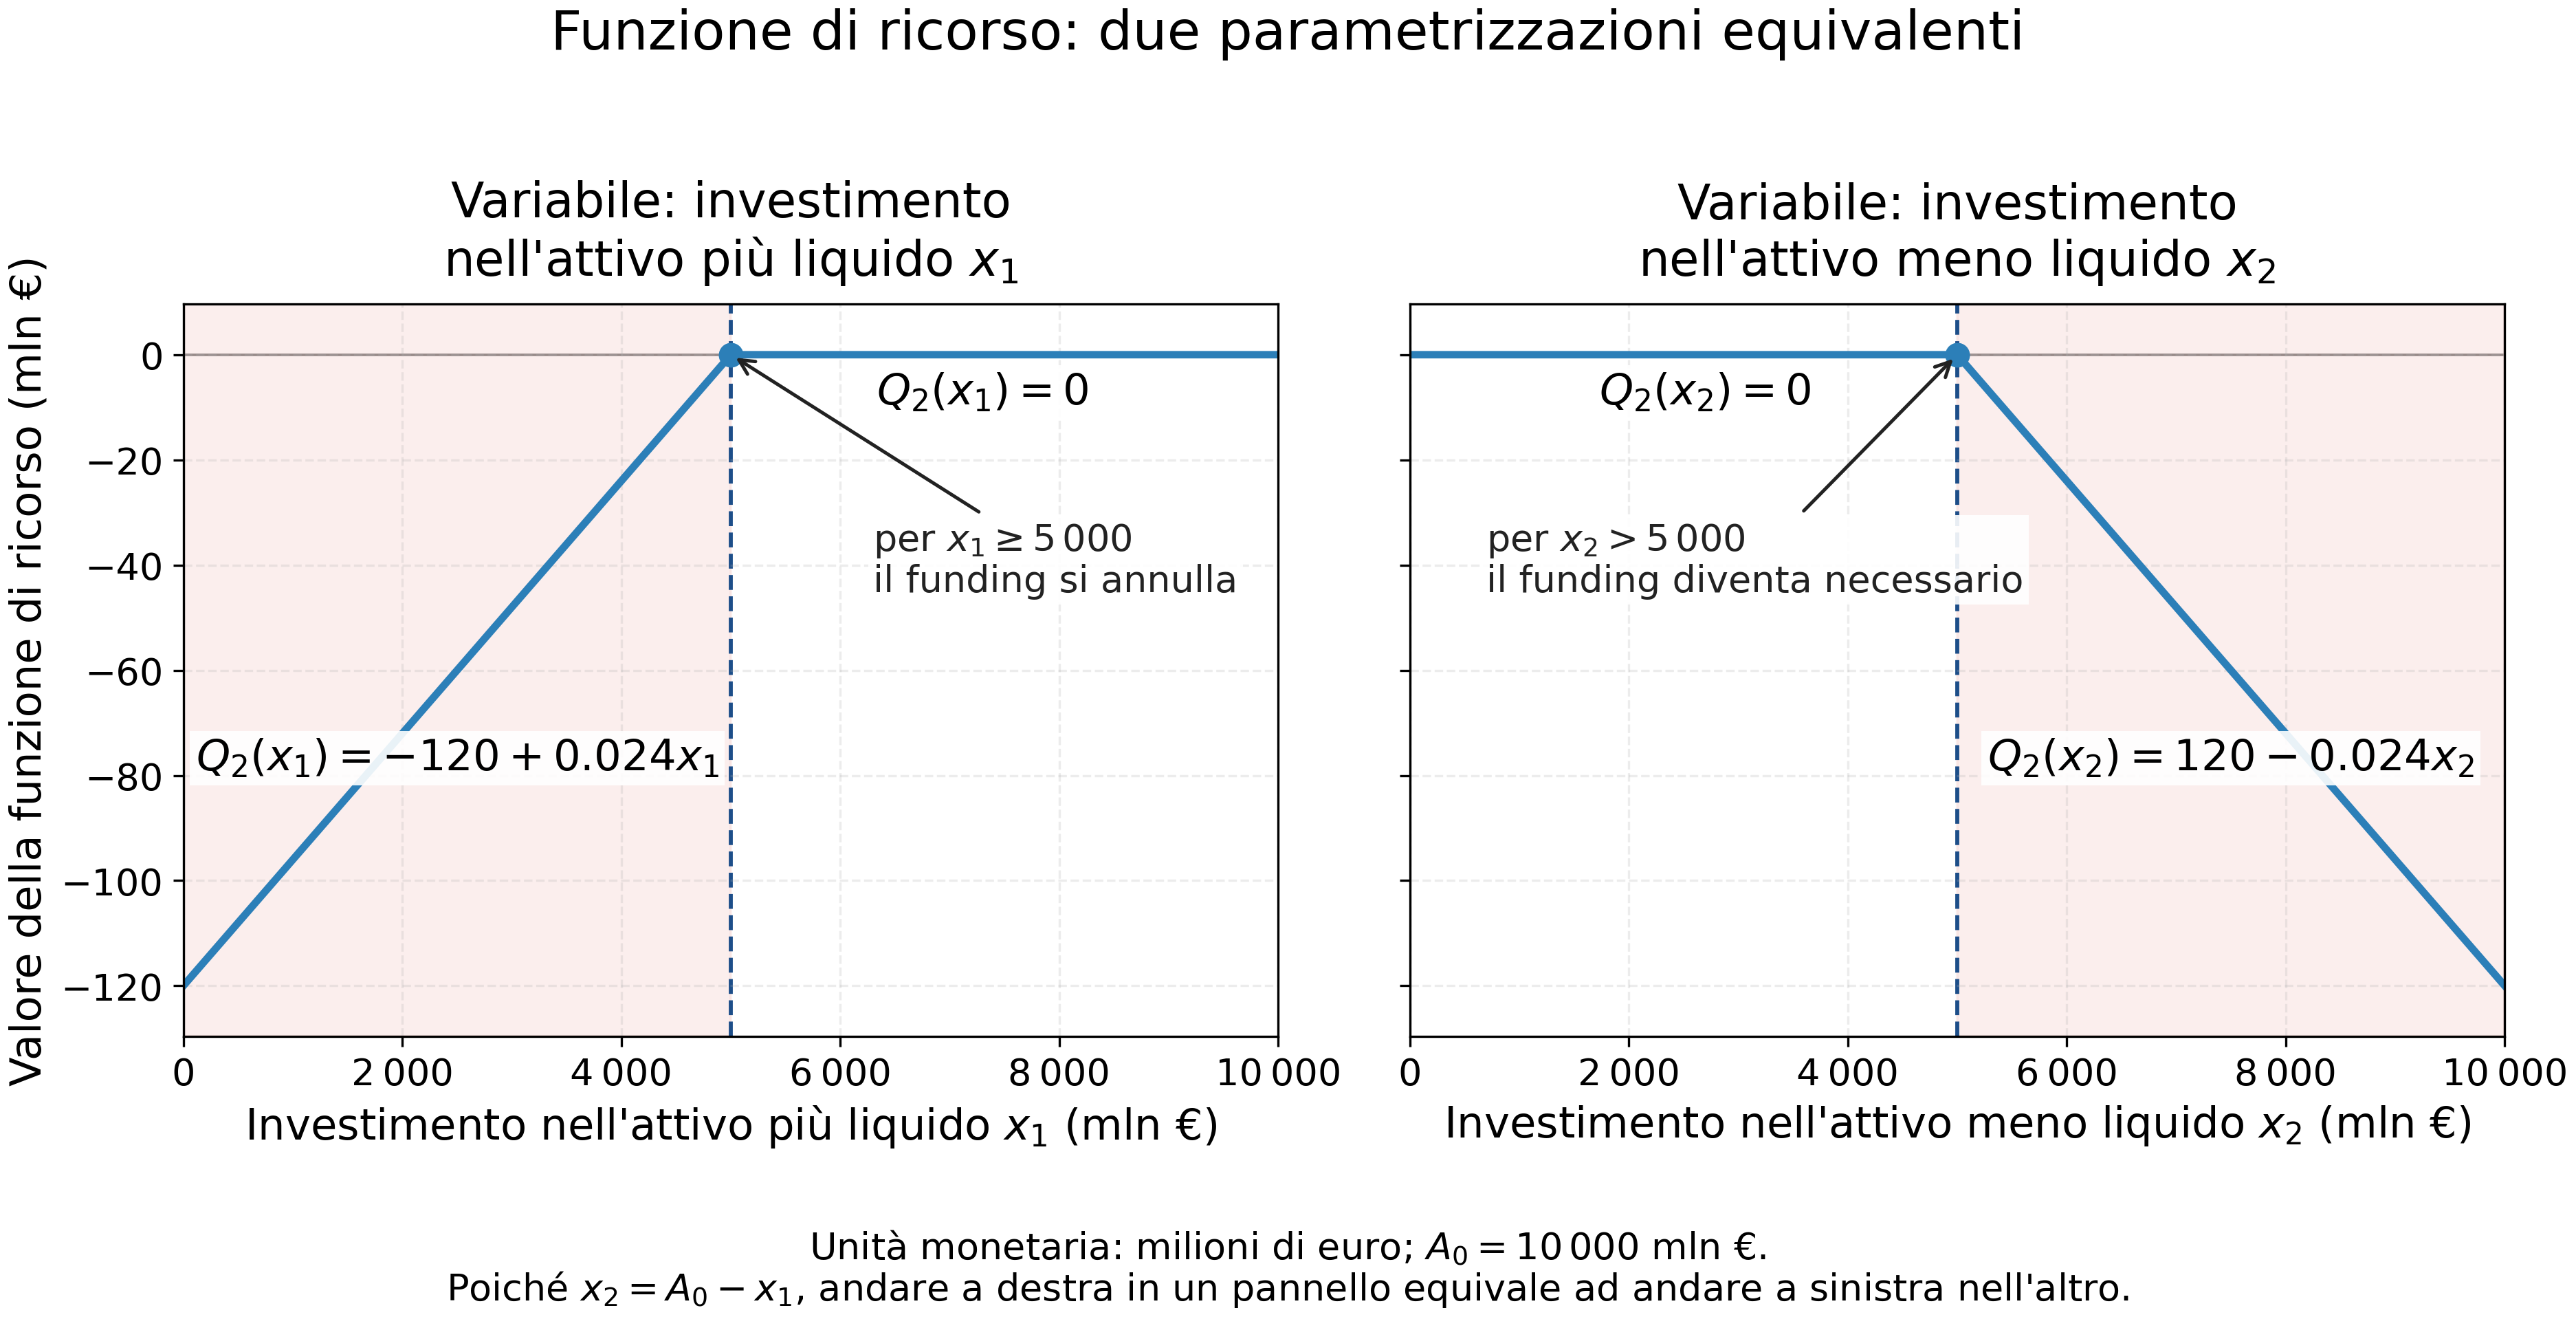
\includegraphics[width=\textwidth]
{../graphics/Cap15_funzione_ricorso_piecewise.png}
\caption{Funzione di ricorso nello scenario avverso secondo due
parametrizzazioni equivalenti della decisione iniziale. Nel pannello di
sinistra la variabile \`e l'investimento $x_1$ nell'attivo pi\`u liquido;
nel pannello di destra \`e l'investimento $x_2$ nell'attivo meno liquido.
Tutte le quantit\`a monetarie sono espresse in milioni di euro e
$A_0=10\,000$.}
\label{fig:cap15-funzione-ricorso-piecewise-v2}
\end{figure}

Le due rappresentazioni descrivono gli stessi portafogli, poich\`e

\[
x_2
=
10\,000-x_1.
\]

Il diverso andamento dei due grafici dipende soltanto dalla variabile scelta
sull'asse orizzontale. Aumentare $x_1$ significa rendere il portafoglio
iniziale pi\`u liquido e ridurre il funding necessario; aumentare $x_2$
produce l'effetto opposto. Per questo $Q_2$ cresce rispetto a $x_1$ e
diminuisce rispetto a $x_2$.

L'esempio rende visibili le due propriet\`a appena introdotte. La funzione di
ricorso \`e lineare all'interno di ciascuna regione e cambia pendenza in

\[
x_1=5\,000
\qquad\text{oppure, equivalentemente,}\qquad
x_2=5\,000,
\]

quando il funding ottimo passa da un valore positivo a zero. Nel problema
generale lo stesso principio opera in dimensione maggiore: al variare della
decisione iniziale possono cambiare le decisioni ottime di secondo stadio e,
con esse, la pendenza della funzione di ricorso.

\section{Perch\`e il modello a due stadi non basta}

\label{sec:cap15-motivazione-multistadio-v2}

Le sezioni precedenti hanno studiato il ricorso nella struttura a due stadi.
La decisione iniziale $x$ viene assunta prima della rivelazione
dell'incertezza; successivamente, dopo avere osservato lo scenario $s$, il
decisore sceglie un unico vettore di ricorso $y_s$.

Nel modello introdotto nel Capitolo~\ref{cap:programmazione-stocastica-due-stadi},
lo scenario $s$ contiene l'intera traiettoria futura rilevante. Il vettore
$y_s$ pu\`o quindi utilizzare tutta l'informazione contenuta nello scenario
ed \`e adattato a

\[
\mathcal F_T.
\]

Questa struttura \`e appropriata quando si vuole distinguere una decisione
iniziale da un unico blocco successivo di decisioni. Diventa invece
restrittiva quando l'informazione rilevante viene resa disponibile
progressivamente e il decisore deve poter modificare le proprie scelte in
pi\`u momenti dell'orizzonte.

Il passaggio al modello multistadio consiste precisamente nel suddividere il
ricorso in pi\`u blocchi decisionali.

\subsection{Stadi decisionali e informazione disponibile}

Nel modello multistadio l'orizzonte successivo alla decisione iniziale \`e
suddiviso in

\[
k=1,\ldots,K
\]

stadi decisionali.

Come stabilito nella Notazione, lo stadio $k$ pu\`o comprendere pi\`u tempi,

\[
\mathcal T_k
=
\{t_{k,1},\ldots,t_{k,n_k}\},
\]

e il suo tempo terminale \`e

\[
\bar t_k
=
t_{k,n_k}.
\]

La decisione di ricorso associata allo stadio $k$ nello scenario $s$ \`e

\[
y_k^s.
\]

Essa viene formulata utilizzando l'informazione disponibile nello stadio e
deve quindi essere adattata a

\[
\mathcal F_{\bar t_k}.
\]

La distinzione fondamentale non \`e quindi tra singole date, ma tra livelli
successivi di informazione. Pi\`u tempi possono appartenere allo stesso
stadio se le corrispondenti decisioni vengono trattate come un unico blocco
rispetto alla struttura informativa del modello.

Nel modello a due stadi esiste un solo blocco di ricorso, adattato
all'informazione completa $\mathcal F_T$. Nel modello multistadio lo stesso
principio viene applicato ripetutamente:

\[
y_1^s
\text{ adattata a }
\mathcal F_{\bar t_1},
\qquad
\ldots,
\qquad
y_K^s
\text{ adattata a }
\mathcal F_{\bar t_K}.
\]

Poich\`e l'ultimo stadio termina con l'orizzonte del problema,

\[
\bar t_K=T,
\]

l'ultima decisione di ricorso pu\`o utilizzare l'informazione completa,
mentre le decisioni precedenti devono rispettare l'informazione disponibile
nei rispettivi stadi.

\subsection{Non anticipativit\`a}

La struttura informativa impone una condizione essenziale. Una decisione non
pu\`o dipendere da informazioni che non sono ancora disponibili nello stadio
in cui essa viene assunta.

\begin{definition}[Decisione adattata alla storia osservata]

\label{def:cap15-decisione-adattata-v2}

La decisione di ricorso $y_k^s$ \`e \emph{adattata} all'informazione
disponibile nello stadio $k$ se \`e
$\mathcal F_{\bar t_k}$-misurabile.

Nella rappresentazione a scenari finiti, se due scenari $s$ e $s'$
condividono la stessa storia informativa fino al tempo $\bar t_k$,
le corrispondenti decisioni devono coincidere:

\begin{equation}
y_k^s=y_k^{s'}
\qquad
\text{se gli scenari }s\text{ e }s'
\text{ hanno la stessa storia fino a }\bar t_k.
\label{eq:cap15-non-anticipativita-multistadio-v2}
\end{equation}

\end{definition}
La condizione~\eqref{eq:cap15-non-anticipativita-multistadio-v2}
esprime il principio di \emph{non anticipativit\`a}.
Due scenari che fino allo stadio $k$ sono
indistinguibili devono produrre la stessa decisione in quello stadio. La
decisione pu\`o differenziarsi soltanto quando sia stata osservata
un'informazione che consente di distinguere le due storie.

Il vincolo di non anticipativit\`a non limita quindi artificialmente la
capacit\`a di adattamento del modello. Impedisce, al contrario, che il
decisore utilizzi informazione futura prima che essa sia disponibile.

\subsection{Dal modello a due stadi al modello multistadio}

Il rapporto tra le due formulazioni pu\`o essere visto con un esempio
astratto.

Supponiamo che l'orizzonte successivo alla decisione iniziale contenga
quattro tempi,

\[
t=1,2,3,4.
\]

Nel modello a due stadi questi quattro tempi appartengono a un unico blocco
di ricorso. Dopo avere osservato l'intero scenario $s$, il decisore sceglie

\[
y_s,
\]

adattato a

\[
\mathcal F_4.
\]

Supponiamo ora di suddividere lo stesso orizzonte in tre stadi:

\[
\mathcal T_1=\{1\},
\qquad
\mathcal T_2=\{2,3\},
\qquad
\mathcal T_3=\{4\}.
\]

I rispettivi tempi terminali sono

\[
\bar t_1=1,
\qquad
\bar t_2=3,
\qquad
\bar t_3=4.
\]

Il ricorso viene allora rappresentato mediante tre decisioni,

\[
y_1^s,
\qquad
y_2^s,
\qquad
y_3^s,
\]

adattate rispettivamente a

\[
\mathcal F_1,
\qquad
\mathcal F_3,
\qquad
\mathcal F_4.
\]

La condizione~\eqref{eq:cap15-non-anticipativita-multistadio-v2}
si applica separatamente a ciascuno dei tre blocchi decisionali.

Se due scenari $s$ e $s'$ coincidono fino al tempo $1$, il primo
blocco decisionale deve soddisfare

\[
y_1^s=y_1^{s'}.
\]

Se le due storie coincidono fino al tempo $3$, deve inoltre valere

\[
y_2^s=y_2^{s'}.
\]

La decisione del terzo stadio \`e invece assunta dopo
l'osservazione dell'intero scenario. Di conseguenza, le decisioni
$y_3^s$ e $y_3^{s'}$ possono differire quando gli scenari completi
sono distinguibili.

L'esempio mostra che il passaggio al multistadio non richiede di modificare
la logica economica del problema. Cambia la struttura informativa con cui le
decisioni di ricorso vengono organizzate. Un unico vettore $y_s$, costruito
conoscendo l'intero scenario, viene sostituito da una sequenza

\[
y_1^s,\ldots,y_K^s,
\]

nella quale ciascuna decisione utilizza soltanto l'informazione disponibile
nel proprio stadio.

Questo rende il modello pi\`u fedele ai problemi nei quali l'incertezza si
rivela progressivamente, ma introduce anche una struttura pi\`u articolata:
le decisioni devono essere associate alle diverse storie informative e
vincolate dalla non anticipativit\`a. Le sezioni successive sviluppano le
rappresentazioni che permettono di organizzare questa struttura.

\section{Il programma stocastico multistadio: formulazione generale}

\label{sec:cap15-programma-multistadio-v2}

La Sezione~\ref{sec:cap15-motivazione-multistadio-v2} ha mostrato come il
ricorso possa essere suddiviso in pi\`u stadi decisionali. In ciascuno
stadio il decisore utilizza l'informazione disponibile in quel momento,
senza conoscere le realizzazioni dell'incertezza appartenenti agli stadi
successivi.

Passiamo ora dalla descrizione della struttura informativa alla
formulazione matematica del programma multistadio. Consideriamo un
insieme finito di scenari completi

\[
\mathcal S=\{1,\ldots,N\},
\]

con probabilit\`a

\[
p_s>0,
\qquad
\sum_{s\in\mathcal S}p_s=1.
\]

Ogni scenario identifica una possibile traiettoria dell'incertezza
sull'intero orizzonte:

\[
\xi_s=(\xi_1^s,\ldots,\xi_T^s).
\]

La decisione iniziale $x$ \`e comune a tutti gli scenari ed \`e assunta
al tempo $t=0$. Le successive decisioni di ricorso sono

\[
y_1^s,\ldots,y_K^s,
\qquad s\in\mathcal S.
\]

Per ogni stadio $k$, il vettore $y_k^s$ viene scelto dopo
l'osservazione dell'intero blocco di incertezza appartenente a
$\mathcal T_k$. Esso pu\`o quindi dipendere dalla storia

\[
(\xi_1^s,\ldots,\xi_{\bar t_k}^s),
\]

ma non dalle realizzazioni successive.

Questa struttura pu\`o essere rappresentata in due modi equivalenti:
mediante decisioni associate alle storie informative, organizzate in
un albero, oppure mediante decisioni distinte per scenario e vincoli
espliciti di non anticipativit\`a.


\subsection{Scenari, storie informative e nodi dell'albero}

Uno scenario completo descrive una traiettoria dell'incertezza
sull'intero orizzonte. Una storia informativa descrive invece
soltanto la parte della traiettoria gi\`a osservata al momento
in cui deve essere assunta una decisione.

Allo stadio $k$, la storia osservata nello scenario $s$ \`e

\[
(\xi_1^s,\ldots,\xi_{\bar t_k}^s).
\]

Due scenari possono avere lo stesso prefisso fino al tempo
$\bar t_k$ e differire nelle realizzazioni successive. In tal
caso il decisore non \`e ancora in grado di distinguerli
quando sceglie la decisione di ricorso dello stadio $k$.

Per organizzare queste relazioni utilizziamo un
\emph{albero degli scenari}. La radice rappresenta il
tempo iniziale $t=0$, quando viene scelta $x$ e l'incertezza
futura non \`e ancora osservata. A ciascuno stadio di
ricorso corrisponde un livello successivo dell'albero.

Un nodo $n$ dello stadio $k$ rappresenta una particolare
storia informativa

\[
(\xi_1,\ldots,\xi_{\bar t_k})
\]

che pu\`o essere osservata al termine dello stadio.

Tutti gli scenari completi che condividono questa storia
attraversano lo stesso nodo. Gli scenari si separano in
nodi differenti soltanto quando le loro storie osservate
diventano diverse.

Ogni nodo diverso dalla radice ha un unico predecessore,
indicato con

\[
a(n).
\]

Il predecessore rappresenta la storia informativa disponibile
al termine dello stadio decisionale precedente.

La probabilit\`a di raggiungere il nodo $n$ \`e

\[
p_n
=
\sum_{\substack{s\in\mathcal S:\\
                 s\text{ attraversa }n}}
p_s.
\]

Pertanto $p_n$ \`e la probabilit\`a complessiva degli scenari
completi compatibili con la storia rappresentata dal nodo.

La somma delle probabilit\`a dei nodi appartenenti a uno stesso
livello \`e pari a uno. Inoltre, per ogni nodo non terminale,
la somma delle probabilit\`a dei suoi figli coincide con la
probabilit\`a del nodo stesso.

Se $n$ \`e figlio di $a(n)$, la probabilit\`a condizionata
di raggiungere $n$, dato che \`e stato raggiunto il suo
predecessore, \`e

\[
\frac{p_n}{p_{a(n)}}.
\]

Il rapporto precedente non coincide in generale con $p_n$:
il primo \`e una probabilit\`a condizionata alla storia
gi\`a osservata, mentre il secondo \`e la probabilit\`a
non condizionata di raggiungere il nodo.

La Figura~\ref{fig:cap15-albero-generico-v2} illustra
un albero con ramificazioni differenti nei diversi nodi.
La costruzione non richiede che da ogni nodo si sviluppi
lo stesso numero di scenari successivi.

\begin{figure}[htbp]
\centering
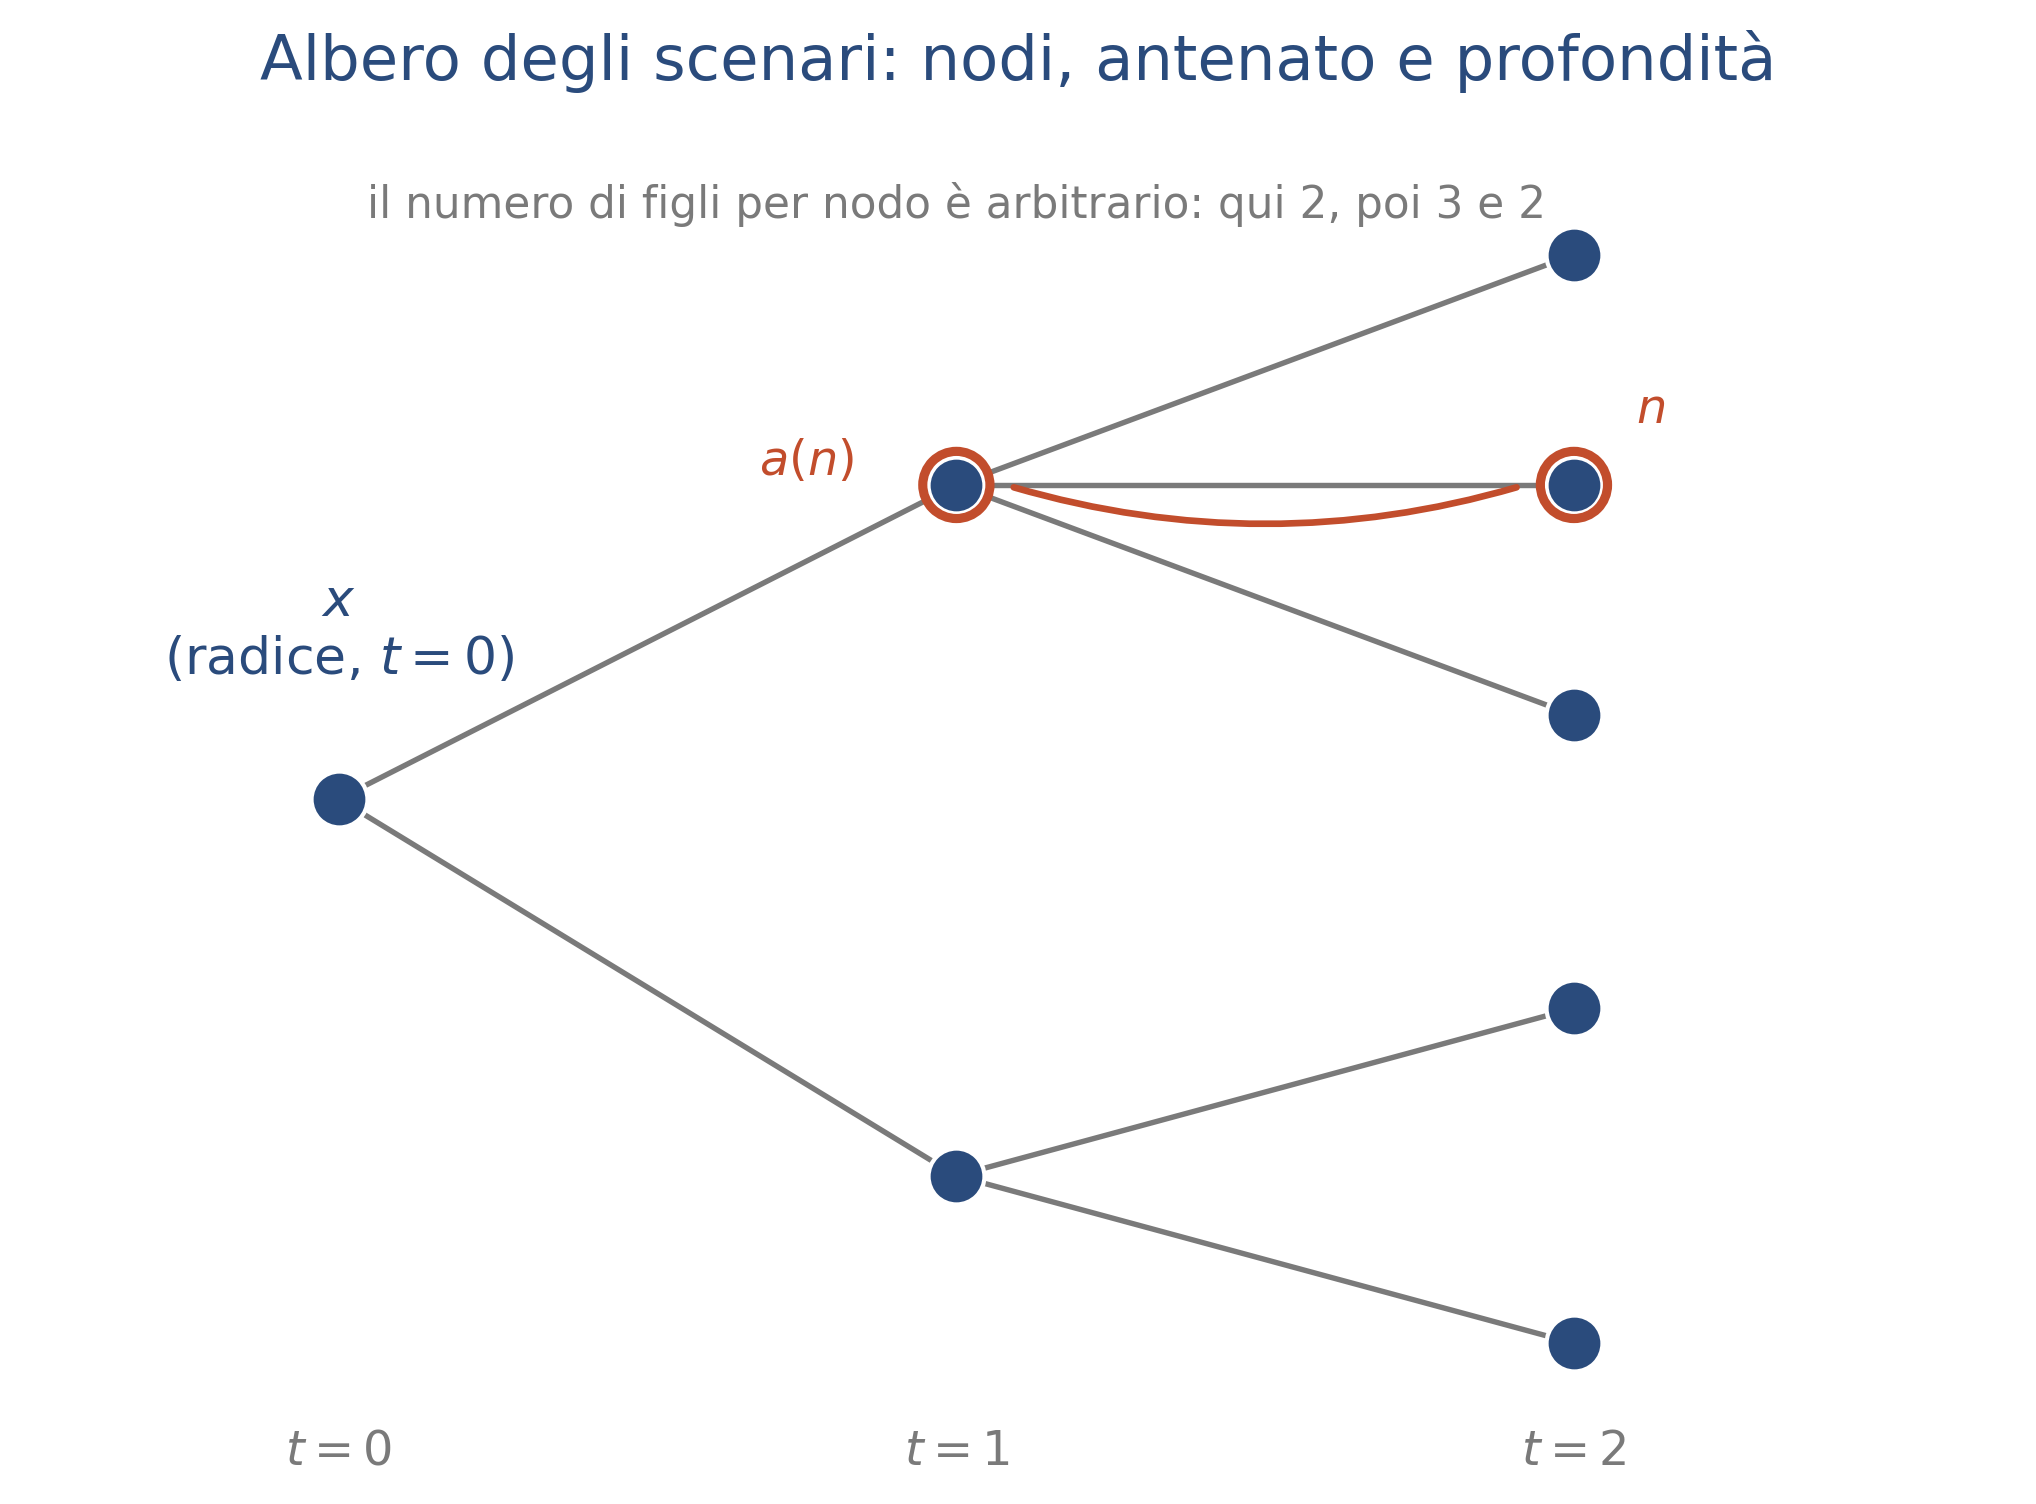
\includegraphics[width=0.7\textwidth]
{../graphics/Cap15_albero_multistadio_generico.png}
\caption{Rappresentazione di un programma stocastico multistadio
mediante un albero degli scenari. Ogni nodo identifica una storia
informativa osservata; i suoi figli rappresentano le possibili
prosecuzioni di quella storia. Il nodo $a(n)$ \`e il predecessore
di $n$. Il numero di ramificazioni pu\`o variare da nodo a nodo.}
\label{fig:cap15-albero-generico-v2}
\end{figure}

\begin{remark}

Nell'albero utilizzato per la formulazione multistadio, i livelli
decisionali sono associati ai tempi terminali degli stadi

\[
\bar t_1,\ldots,\bar t_K.
\]

Se uno stadio comprende pi\`u tempi fisici, il passaggio al livello
successivo dell'albero incorpora l'osservazione dell'intero blocco
di incertezza compreso in quello stadio.

Non occorre introdurre un nuovo stadio decisionale per ogni tempo
fisico: la partizione dell'orizzonte in stadi resta quella definita
nella Sezione~\ref{sec:cap15-motivazione-multistadio-v2}.

\end{remark}


\subsection{Non anticipativit\`a implicita ed esplicita}

L'albero permette di rappresentare direttamente il principio di
non anticipativit\`a introdotto nella
Definizione~\ref{def:cap15-decisione-adattata-v2}.

Consideriamo un nodo $n$ appartenente allo stadio $k$.
In tale nodo il decisore dispone della storia osservata
fino al tempo $\bar t_k$. Alla storia rappresentata dal
nodo associamo un unico vettore decisionale

\[
y_n.
\]

Questo vettore \`e utilizzato da tutti gli scenari completi
che attraversano il nodo $n$.

Se due scenari $s$ e $s'$ coincidono fino al tempo
$\bar t_k$, essi attraversano lo stesso nodo dello
stadio $k$. La decisione assegnata a entrambi \`e
quindi necessariamente la stessa.

L'indicizzazione per nodo soddisfa pertanto la
non anticipativit\`a per costruzione: non \`e
necessario introdurre ulteriori uguaglianze fra
decisioni che appartengono alla stessa storia informativa.

Questa \`e la rappresentazione \emph{implicita}
della non anticipativit\`a.

Un'alternativa consiste nel conservare, come nella
formulazione a due stadi del
Capitolo~\ref{cap:programmazione-stocastica-due-stadi},
una copia delle decisioni di ricorso per ogni
scenario completo:

\[
y_k^s,
\qquad
k=1,\ldots,K,
\quad
s\in\mathcal S.
\]

In questo caso le decisioni dei diversi scenari sono
inizialmente variabili distinte del programma matematico.
Occorre quindi imporre esplicitamente

\begin{equation}
y_k^s=y_k^{s'}
\quad
\text{se}
\quad
(\xi_1^s,\ldots,\xi_{\bar t_k}^s)
=
(\xi_1^{s'},\ldots,\xi_{\bar t_k}^{s'}),
\label{eq:cap15-non-anticipativita-multistadio-v2}
\end{equation}

per ogni stadio $k$ e per ogni coppia di scenari
con la stessa storia fino al termine dello stadio.

Questa \`e la rappresentazione \emph{esplicita}
della non anticipativit\`a.

Le due rappresentazioni producono lo stesso insieme
di decisioni ammissibili dal punto di vista informativo.
La corrispondenza \`e immediata: se lo scenario $s$
attraversa il nodo $n$ dello stadio $k$, si pone

\[
y_k^s=y_n.
\]

Viceversa, le uguaglianze
\eqref{eq:cap15-non-anticipativita-multistadio-v2}
garantiscono che tutte le copie scenario-specifiche
associate al medesimo nodo abbiano lo stesso valore.
A tale valore comune pu\`o essere associata
un'unica variabile $y_n$.

L'equivalenza non richiede che le decisioni di nodi
differenti siano necessariamente diverse: due storie
distinguibili possono comunque condurre, per ragioni
economiche o operative, alla stessa scelta ottima.

\begin{remark}

La condizione di non anticipativit\`a riguarda l'intero
vettore $y_k^s$, non soltanto alcune sue componenti.
Se due scenari hanno la stessa storia fino a
$\bar t_k$, devono coincidere tutte le componenti
del blocco decisionale dello stadio $k$.

La coincidenza delle sole osservazioni riferite
all'ultimo tempo dello stadio,

\[
\xi_{\bar t_k}^s=\xi_{\bar t_k}^{s'},
\]

non \`e invece sufficiente, in generale, per imporre
l'uguaglianza delle decisioni: le due storie precedenti
potrebbero essere differenti.

\end{remark}


\subsection{Forma estesa generale}

La rappresentazione per scenari consente di riunire
in un unico problema di ottimizzazione la decisione
iniziale e tutte le decisioni di ricorso successive.

Consideriamo un programma stocastico lineare formulato
in massimizzazione. Manteniamo $c'x$ come contributo
della decisione iniziale e indichiamo con

\[
(q_k^s)'y_k^s
\]

il contributo lineare attribuito al blocco decisionale
dello stadio $k$ nello scenario $s$.

Assumiamo che i coefficienti economici e i dati dei
vincoli propri dello stadio $k$ siano determinati
dall'informazione disponibile fino a $\bar t_k$.
Eventuali conseguenze economiche che si manifestano
soltanto negli stadi successivi vengono contabilizzate
nei corrispondenti contributi futuri.

Il valore complessivo nello scenario $s$ \`e
quindi

\[
c'x+\sum_{k=1}^{K}(q_k^s)'y_k^s.
\]

L'obiettivo del programma stocastico \`e massimizzarne
il valore atteso:

\[
c'x+
\sum_{s\in\mathcal S}
p_s\sum_{k=1}^{K}(q_k^s)'y_k^s.
\]

Occorre inoltre rappresentare i vincoli che collegano
le decisioni assunte nei diversi stadi.

Nel caso lineare, i vincoli relativi allo stadio $k$
possono dipendere dalla decisione iniziale $x$ e
dalle decisioni di ricorso assunte fino a quello stadio.
Una scrittura generale, con vincoli di uguaglianza, \`e

\[
T_k^s x+
\sum_{j=1}^{k}W_{k,j}^s y_j^s
=
h_k^s.
\]

Le matrici $T_k^s$ e $W_{k,j}^s$ e il vettore
$h_k^s$ descrivono i dati dei vincoli dello stadio
$k$ nello scenario $s$. Il termine
$W_{k,j}^s y_j^s$ rappresenta l'effetto di una
decisione assunta nello stadio $j$ sui vincoli
dello stadio $k$.

La somma comprende soltanto gli stadi

\[
j=1,\ldots,k:
\]

i vincoli dello stadio corrente non dipendono da
decisioni che saranno assunte in stadi successivi.

Indichiamo con $\mathcal X$ l'insieme delle decisioni
iniziali ammissibili e con $\mathcal X_k^s$
l'insieme degli eventuali vincoli operativi propri
del blocco decisionale $y_k^s$.

La \emph{forma estesa} del programma stocastico
multistadio pu\`o allora essere scritta come

\begin{equation}
\begin{aligned}
\max_{x,\{y_k^s\}}
\quad&
c'x+
\sum_{s\in\mathcal S}
p_s\sum_{k=1}^{K}(q_k^s)'y_k^s
\\[4pt]
\text{soggetto a}\quad&
x\in\mathcal X,
\\[4pt]
&
T_k^s x+
\sum_{j=1}^{k}W_{k,j}^s y_j^s
=
h_k^s,
\qquad
k=1,\ldots,K,
\quad s\in\mathcal S,
\\[4pt]
&
y_k^s\in\mathcal X_k^s,
\qquad
k=1,\ldots,K,
\quad s\in\mathcal S,
\\[4pt]
&
y_k^s=y_k^{s'}
\quad
\text{se}\quad
(\xi_1^s,\ldots,\xi_{\bar t_k}^s)
=
(\xi_1^{s'},\ldots,\xi_{\bar t_k}^{s'}),
\\[-1pt]
&
\hspace{2.1cm}
k=1,\ldots,K,
\quad s,s'\in\mathcal S.
\end{aligned}
\label{eq:cap15-forma-estesa-multistadio-v2}
\end{equation}

Le uguaglianze considerate rappresentano i vincoli
lineari di collegamento tra le decisioni. Quando il
modello economico richiede disuguaglianze, limiti
di capacit\`a o altre condizioni lineari,
queste possono essere incluse negli insiemi
di ammissibilit\`a oppure aggiunte esplicitamente
al sistema.

La formulazione
\eqref{eq:cap15-forma-estesa-multistadio-v2}
contiene tre elementi distinti.

La decisione iniziale $x$ compare una sola volta:
il decisore non pu\`o scegliere un portafoglio
iniziale diverso in funzione dello scenario
che si realizzer\`a successivamente.

Le decisioni $y_k^s$ sono invece replicate per
scenario e per stadio. Questa replicazione permette
di rappresentare tutti i possibili adattamenti
futuri alle diverse realizzazioni dell'incertezza.

Infine, i vincoli di non anticipativit\`a
collegano le copie delle decisioni che, al
momento della scelta, dispongono della stessa
informazione.

Senza tali vincoli, le decisioni
scenario-specifiche potrebbero differire
anche tra scenari che non sono ancora
distinguibili. Si otterrebbe quindi un
problema con possibilit\`a decisionali
pi\`u ampie di quelle effettivamente
consentite dalla struttura informativa
del modello.

\medskip

\noindent
\textbf{Forma estesa con decisioni associate ai nodi.}

La stessa struttura pu\`o essere rappresentata
utilizzando un'unica decisione $y_n$ per ogni nodo
informativo.

Sotto l'ipotesi che i coefficienti economici dello
stadio siano determinati dalla storia rappresentata
dal nodo, al nodo $n$ corrisponde un vettore
di coefficienti $q_n$.

Il contributo atteso delle decisioni di ricorso
pu\`o allora essere scritto come

\[
\sum_n p_n q_n'y_n,
\]

dove la somma \`e estesa ai nodi decisionali
successivi alla radice.

Infatti, la probabilit\`a del nodo $n$ \`e
la somma delle probabilit\`a di tutti gli
scenari che lo attraversano. Poich\`e tali
scenari condividono sia la decisione $y_n$
sia il relativo contributo economico dello
stadio, sommare i contributi per scenario
oppure per nodo produce lo stesso valore atteso.

Anche i vincoli possono essere organizzati
per nodo e per storia antecedente. In questa
rappresentazione la non anticipativit\`a
\`e incorporata nella scelta di un'unica
variabile decisionale per ogni nodo.

La forma estesa per scenari e la forma estesa
per nodi descrivono dunque lo stesso problema
decisionale. Esse differiscono nel modo in
cui organizzano le variabili e i vincoli,
non nell'informazione che il decisore
pu\`o utilizzare.


\subsection{Raccordo con il modello a due stadi}

Verifichiamo infine che la formulazione
multistadio comprenda come caso particolare
il programma a due stadi introdotto nel
Capitolo~\ref{cap:programmazione-stocastica-due-stadi}.

Supponiamo che l'intero orizzonte successivo
alla decisione iniziale appartenga a un
unico stadio di ricorso:

\[
K=1,
\qquad
\mathcal T_1=\{1,\ldots,T\},
\qquad
\bar t_1=T.
\]

Il vettore $y_1^s$ viene scelto dopo
l'osservazione dell'intero scenario

\[
\xi_s=(\xi_1^s,\ldots,\xi_T^s)
\]

ed \`e quindi adattato a $\mathcal F_T$.

Non esistono decisioni di ricorso intermedie.
La forma estesa
\eqref{eq:cap15-forma-estesa-multistadio-v2}
si riduce a

\[
\begin{aligned}
\max_{x,\{y_1^s\}}
\quad&
c'x+
\sum_{s\in\mathcal S}
p_s(q_1^s)'y_1^s
\\
\text{soggetto a}\quad&
x\in\mathcal X,
\\
&
T_1^s x+W_{1,1}^s y_1^s=h_1^s,
\qquad s\in\mathcal S,
\\
&
y_1^s\in\mathcal X_1^s,
\qquad s\in\mathcal S.
\end{aligned}
\]

Se gli scenari completi sono distinti, non
occorrono ulteriori uguaglianze tra le
decisioni di ricorso: una volta osservato
l'intero scenario, il decisore dispone
dell'informazione necessaria per distinguerlo
dagli altri.

Riprendendo la notazione del Capitolo 14,

\[
y_1^s=y_s,
\qquad
q_1^s=q_s,
\qquad
T_1^s=T_s,
\qquad
W_{1,1}^s=W_s,
\qquad
h_1^s=h_s,
\]

si ottiene

\[
\max_{x,\{y_s\}}
\left\{
c'x+
\sum_{s\in\mathcal S}p_s q_s'y_s
\right\},
\]

soggetto a

\[
x\in\mathcal X,
\]

\[
T_sx+W_sy_s=h_s,
\qquad
y_s\in\mathcal X_s,
\qquad
s\in\mathcal S.
\]

Questa \`e precisamente la forma estesa
del programma stocastico a due stadi
presentata nella
\eqref{eq:cap14-forma-estesa}.

La differenza tra le due formulazioni
non consiste pertanto nell'introdurre
un diverso tipo di problema di ricorso.
Nel modello a due stadi tutte le
decisioni correttive sono raccolte in
un unico vettore scelto dopo
l'osservazione dello scenario completo;
nel modello multistadio il ricorso
\`e suddiviso in pi\`u blocchi,
ciascuno vincolato all'informazione
disponibile nel momento in cui
viene assunto.

La formulazione generale \`e ora
disponibile. Nella sezione successiva
la specializzeremo al caso SVB--ALM,
identificando le decisioni iniziali,
i blocchi di ricorso e i vincoli
finanziari che collegano gli stadi.